\documentclass[aspectratio=169,xcolor=dvipsnames]{beamer}
\usetheme{SimpleDarkBlue}
\usepackage[T5]{fontenc}
\usepackage[utf8]{inputenc}
\usepackage{hyperref}
\usepackage{graphicx}
\graphicspath{{images/}}
\usepackage{booktabs}
\usepackage{listings}
\usepackage{color}
\usepackage[numbers]{natbib}
\definecolor{dkgreen}{rgb}{0,0.6,0}
\definecolor{gray}{rgb}{0.5,0.5,0.5}
\definecolor{mauve}{rgb}{0.58,0,0.82}
\lstset{frame=tb,aboveskip=2mm,belowskip=2mm,
 showstringspaces=false,columns=fullflexible,
 basicstyle=\small\ttfamily,numbers=none,
 commentstyle=\color{dkgreen},stringstyle=\color{mauve},
 breaklines=true,breakatwhitespace=false,tabsize=2}
\title{Movie Knowledge Graph}
\subtitle{A Linked Open Data Application}
\author[Do Tuan Hoang \and Nguyen Truong Huy]{%
  \begin{tabular}{c@{\hspace{1.5em}}c}
    Do Tuan Hoang & Nguyen Truong Huy \\
    {\small 20261219M} & {\small 20261260M} \\
    {\scriptsize\href{mailto:Hoang.DT261219M@sis.hust.edu.vn}{Hoang.DT261219M@sis.hust.edu.vn}} &
    {\scriptsize\href{mailto:Huy.NT261260M@sis.hust.edu.vn}{Huy.NT261260M@sis.hust.edu.vn}}
  \end{tabular}%
}
% \institute{Institution}
\date{\today}
\begin{document}
\begin{frame}
\titlepage
\end{frame}

%------------------------------------------------
\begin{frame}{Outline}
\tableofcontents
\end{frame}

%------------------------------------------------

\section{Define an ontology for the movie domain}

\begin{frame}{Outline}
    \tableofcontents[currentsection]
\end{frame}

%------------------------------------------------

\begin{frame}{Define an ontology: overview}
\centering
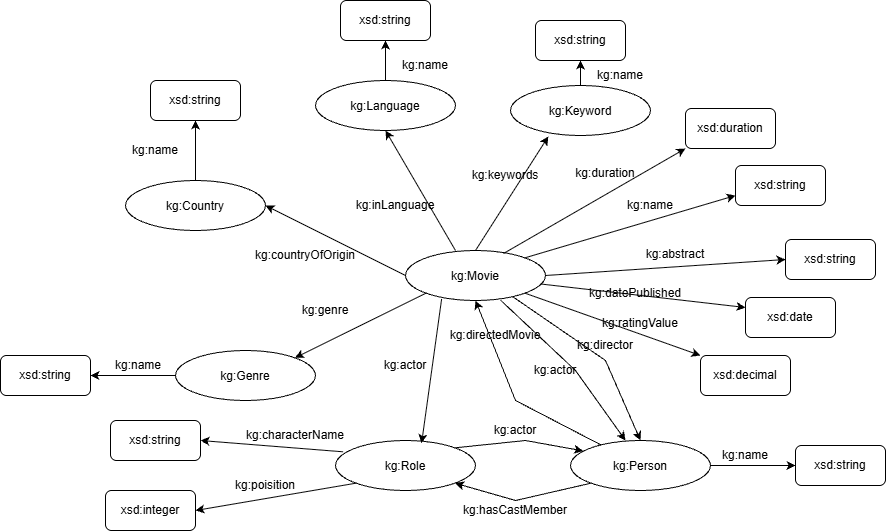
\includegraphics[width=.94\linewidth,height=.77\textheight,keepaspectratio]{ontology.png}
\end{frame}

%------------------------------------------------

\begin{frame}{Define an ontology: classes and instances}
\small
All domain terms use \texttt{kg:} = \url{https://example.org/ontology/}.
\medskip
\begin{itemize}
\item \textbf{Movie}: Iron Man 2, identified by TMDB ID 10138.
\item \textbf{Person}: a shared actor or director resource.
\item \textbf{Role}: one acting participation, with character and cast order.
\item \textbf{Genre}: Drama, Action, and other genre instances.
\item \textbf{Country}: countries associated with movie production.
\item \textbf{Language}: original and spoken languages.
\item \textbf{Keyword}: descriptive terms shared by movies.
\end{itemize}
\medskip
A class is a category; an instance is a particular member of that category.
\end{frame}

%------------------------------------------------

\begin{frame}{Define an ontology: properties and literals}
\small
\textbf{Object properties connect resources}
\begin{itemize}
\item Movie relationships: \texttt{actor}, \texttt{director}, \texttt{genre},
\texttt{keywords}, \texttt{countryOfOrigin}, \texttt{inLanguage}.
\item Role to person: \texttt{actor}; movie to webpage: \texttt{referencePage}.
\item Reasoning relationships: \texttt{directedMovie}, \texttt{hasCastMember}.
\end{itemize}
\medskip
\textbf{Datatype properties connect resources to literal values}
\begin{itemize}
\item \texttt{name}, \texttt{abstract}, \texttt{characterName}: strings.
\item \texttt{datePublished}: date; \texttt{duration}: duration.
\item \texttt{position}: integer; \texttt{ratingValue}: decimal.
\end{itemize}
\end{frame}

%------------------------------------------------

\begin{frame}[fragile]{Define an ontology: restrictions and reasoning}
\small
\begin{itemize}
\item The seven classes are disjoint.
\item Movie: at least one name; at most one rating value.
\item Role: exactly one actor of type Person; at most one character name and position.
\end{itemize}
\begin{lstlisting}
kg:directedMovie owl:inverseOf kg:director .
kg:hasCastMember owl:propertyChainAxiom
  (kg:directedMovie kg:actor) .
\end{lstlisting}
\texttt{Person -> directedMovie -> Movie -> actor -> Person/Role}
\medskip

The chain derives \texttt{hasCastMember}. Missing-field checks are separate from OWL reasoning.
\end{frame}

%------------------------------------------------

\section{Collect relevant data in the movie domain}

\begin{frame}{Outline}
    \tableofcontents[currentsection]
\end{frame}

%------------------------------------------------

\begin{frame}{Collect relevant data in the movie domain}
\begin{itemize}
\item \textbf{Original data:}
\href{https://www.kaggle.com/datasets/tmdb/tmdb-movie-metadata}{TMDB 5000 Movie Dataset on Kaggle}.
Movie metadata and credits in two CSV files.
\medskip
\item \textbf{Processed data:} \textit{[Insert our processed-dataset link here]}.
100 movies, up to ten cast members per movie, directors only; eleven CSV tables.
\medskip
\item \textbf{External data:}
\href{https://www.wikidata.org/}{Wikidata} and
\href{https://www.dbpedia.org/}{DBpedia} for linking local resources.
\end{itemize}
\end{frame}

%------------------------------------------------

\section{Transform collected data into 4-star RDF}

\begin{frame}{Outline}
    \tableofcontents[currentsection]
\end{frame}

%------------------------------------------------

\begin{frame}[fragile]{Transform collected data: stable identifiers}
Each entity receives a URI based on its type and source ID.
\begin{lstlisting}
Movie ID 10138:
https://example.org/movie/10138

Person ID 3223:
https://example.org/person/3223

Genre ID 28:
https://example.org/genre/28
\end{lstlisting}
The same person URI is reused across movies and credits.
Titles are display values, while source IDs identify resources.
\end{frame}

%------------------------------------------------

\begin{frame}[fragile]{Transform collected data: RDF triples}
\small
A movie becomes a resource with relationships and typed literals~\cite{w3c2014rdf11}.
\begin{lstlisting}
@prefix kg: <https://example.org/ontology/> .
@prefix xsd: <http://www.w3.org/2001/XMLSchema#> .

<https://example.org/movie/10138>
  a kg:Movie ;
  kg:name "Iron Man 2" ;
  kg:datePublished "2010-04-28"^^xsd:date ;
  kg:genre <https://example.org/genre/28> .
\end{lstlisting}
\textbf{Output:} 100 movies and 11,603 triples in \texttt{movies.ttl}.
\medskip

This implements URI-based RDF. Public deployment still needs persistent,
resolvable URIs in place of \texttt{example.org}.
\end{frame}

%------------------------------------------------

\section{Establish links to other datasets}

\begin{frame}{Outline}
    \tableofcontents[currentsection]
\end{frame}

%------------------------------------------------

\begin{frame}{Establish links: matching strategy}
\small
A script finds links automatically by querying Wikidata with SPARQL.
\medskip

\begin{itemize}
\item \textbf{Movie:} TMDB ID $\rightarrow$ title + year $\rightarrow$ manual check
\item \textbf{Person:} TMDB ID $\rightarrow$ name in cast/director of a linked film $\rightarrow$ manual check
\item \textbf{Country:} ISO 3166-1 code
\item \textbf{Language:} ISO 639-1 code
\item \textbf{Genre:} film-genre label + synonym $\rightarrow$ manual check
\begin{itemize}
\item e.g. ``Action'' $\rightarrow$ ``action film'', ``Animation'' $\rightarrow$ ``animated film''
\end{itemize}
\end{itemize}
\medskip
IDs are exact, so they come first; names are ambiguous.\\
Unmatched or ambiguous cases are verified by hand on Wikidata.
\end{frame}

%------------------------------------------------

\begin{frame}[fragile]{Establish links: represent with \texttt{owl:sameAs}}
\small
Links connect our resources to other datasets~\cite{bernerslee2006linkeddata}.
\begin{lstlisting}
<.../movie/10138>
  owl:sameAs <http://www.wikidata.org/entity/Q205028> ,
             <http://dbpedia.org/resource/Iron_Man_2> .

<.../genre/28>
  skos:closeMatch <http://www.wikidata.org/entity/Q188473> .
\end{lstlisting}
\begin{itemize}
\item Genres use the weaker \texttt{skos:closeMatch}.
\item 99 movies, 805 people, and 56 lookup resources approved.
\item \textbf{1,901} link triples in total.
\end{itemize}
External links provide the cross-dataset connection for the fifth star.
\end{frame}

%------------------------------------------------

\section{Provide a SPARQL query interface}

\begin{frame}{Outline}
    \tableofcontents[currentsection]
\end{frame}

%------------------------------------------------

\begin{frame}[fragile]{Interface via SPARQL endpoint/terminal to query data}
\small
Our terminal interface loads movie data, the ontology, and optional link files.
SPARQL selects matching graph patterns~\cite{w3c2013sparql}.
\begin{lstlisting}
python scripts/ask.py -q queries/4.sparql

python scripts/ask.py -q queries/11.sparql --reasoning

python scripts/ask.py -q queries/show_links.sparql
  --links output/movie_links.ttl
\end{lstlisting}
The last example is one command, wrapped here for display.
\texttt{--reasoning} adds inferred triples before the query runs.
\end{frame}

%------------------------------------------------

\begin{frame}[fragile]{Interface via SPARQL endpoint/terminal to query data}
\small
Do we have any Spider-Man movies?
\begin{lstlisting}[basicstyle=\footnotesize\ttfamily]
PREFIX kg: <https://example.org/ontology/>

SELECT ?movie ?title WHERE {
  ?movie a kg:Movie ; kg:name ?title .
  FILTER(CONTAINS(LCASE(STR(?title)), "spider"))
}
ORDER BY ?title
\end{lstlisting}
\footnotesize No reasoning needed.
\end{frame}

%------------------------------------------------

\begin{frame}[fragile]{Interface via SPARQL endpoint/terminal to query data}
\small
Who acted in Avatar, and which characters did they play?
\begin{lstlisting}[basicstyle=\footnotesize\ttfamily]
PREFIX kg: <https://example.org/ontology/>
SELECT ?person ?name ?character ?position WHERE {
  VALUES ?movie { <https://example.org/movie/19995> }
  ?movie kg:actor ?role .
  ?role a kg:Role ; kg:actor ?person ; kg:position ?position .
  ?person a kg:Person ; kg:name ?name .
  OPTIONAL { ?role kg:characterName ?character }
}
ORDER BY ?position ?name
LIMIT 10
\end{lstlisting}
\footnotesize Follows Movie -> Role -> Person.
\end{frame}

%------------------------------------------------

\begin{frame}[fragile]{Interface via SPARQL endpoint/terminal to query data}
\small
Which Drama films have the highest average rating?
\begin{lstlisting}[basicstyle=\footnotesize\ttfamily]
PREFIX kg: <https://example.org/ontology/>
SELECT ?movie ?title ?average WHERE {
  ?movie a kg:Movie ;
         kg:name ?title ;
         kg:genre ?genre ;
         kg:ratingValue ?average .
  ?genre kg:name "Drama" .
}
ORDER BY DESC(?average) ?title
LIMIT 20
\end{lstlisting}
\footnotesize Ratings are decimal values directly on movies.
\end{frame}

%------------------------------------------------

\begin{frame}[fragile]{Interface via SPARQL endpoint/terminal to query data}
\small
Which Action films since 2010 feature Scarlett Johansson?
\begin{lstlisting}[basicstyle=\footnotesize\ttfamily]
PREFIX kg: <https://example.org/ontology/>
PREFIX xsd: <http://www.w3.org/2001/XMLSchema#>
SELECT DISTINCT ?movie ?title ?date WHERE {
  VALUES ?actor { <https://example.org/person/1245> }
  VALUES ?genreName { "Action" }
  ?movie a kg:Movie ; kg:name ?title ; kg:datePublished ?date ;
         kg:actor ?actor ; kg:genre ?genre .
  ?actor a kg:Person .
  ?genre kg:name ?genreName .
  FILTER (?date >= "2010-01-01"^^xsd:date)
}
ORDER BY ?date ?title
\end{lstlisting}
\footnotesize Combines actor, genre, and release-date conditions.
\end{frame}

%------------------------------------------------

\begin{frame}[fragile]{Interface via SPARQL endpoint/terminal to query data}
\small
Which directors have at least two movies in our sample?
\begin{lstlisting}[basicstyle=\footnotesize\ttfamily]
PREFIX kg: <https://example.org/ontology/>
SELECT ?director ?name (COUNT(DISTINCT ?movie) AS ?films) WHERE {
  ?movie a kg:Movie ; kg:director ?director .
  ?director a kg:Person ; kg:name ?name .
}
GROUP BY ?director ?name
HAVING (COUNT(DISTINCT ?movie) >= 2)
ORDER BY DESC(?films) ?name
\end{lstlisting}
\footnotesize Uses grouping and counting.
\end{frame}

%------------------------------------------------

\begin{frame}[fragile]{Interface via SPARQL endpoint/terminal to query data}
\small
Which movies did each person direct?
\begin{lstlisting}[basicstyle=\footnotesize\ttfamily]
PREFIX kg: <https://example.org/ontology/>
SELECT ?director ?name ?movie ?title WHERE {
  ?director kg:directedMovie ?movie ; kg:name ?name .
  ?movie kg:name ?title .
}
ORDER BY ?name ?title
LIMIT 20
\end{lstlisting}
\footnotesize Run with --reasoning: uses the inverse of kg:director.
\end{frame}

%------------------------------------------------

\begin{frame}[fragile]{Interface via SPARQL endpoint/terminal to query data}
\small
Which actors appeared in movies directed by each person?
\begin{lstlisting}[basicstyle=\footnotesize\ttfamily]
PREFIX kg: <https://example.org/ontology/>
SELECT DISTINCT ?director ?directorName ?actor ?actorName WHERE {
  ?director kg:hasCastMember ?actor ; kg:name ?directorName .
  ?actor a kg:Person ; kg:name ?actorName .
}
ORDER BY ?directorName ?actorName
\end{lstlisting}
\footnotesize Run with --reasoning: uses the property chain.
\end{frame}

%------------------------------------------------

\begin{frame}[fragile]{Interface via SPARQL endpoint/terminal to query data}
\small
Which external resources are linked to our movies?
\begin{lstlisting}[basicstyle=\footnotesize\ttfamily]
PREFIX kg: <https://example.org/ontology/>
PREFIX owl: <http://www.w3.org/2002/07/owl#>

SELECT ?title ?external WHERE {
  ?movie a kg:Movie ;
         kg:name ?title ;
         owl:sameAs ?external .
}
ORDER BY ?title
\end{lstlisting}
\footnotesize Load --links output/movie\_links.ttl; reasoning is not required.
\end{frame}

%------------------------------------------------


\begin{frame}[fragile]{Interface via SPARQL endpoint/terminal to query data}
\small
Which keywords describe Iron Man 2?
\begin{lstlisting}[basicstyle=\footnotesize\ttfamily]
PREFIX kg: <https://example.org/ontology/>
SELECT ?keywordName WHERE {
  <https://example.org/movie/10138>
    kg:keywords ?keyword .
  ?keyword kg:name ?keywordName .
}
ORDER BY ?keywordName
\end{lstlisting}
\footnotesize Demonstrates our keyword extension; no reasoning needed.
\end{frame}

%------------------------------------------------

\begin{frame}[allowframebreaks]{References}
\footnotesize
\bibliographystyle{plainnat}
\bibliography{reference}
\end{frame}

%------------------------------------------------

% Add your Fuseki appendix here.
\end{document}
